\documentclass[12pt]{article}
\usepackage{amsmath, amsthm, amsfonts, amssymb, amscd, bm}
% \usepackage{apalike}  % citation
\usepackage{appendix}

\usepackage[utf8]{inputenc}
\usepackage[english]{babel}
% \usepackage[backend=biber, style=numeric]{biblatex}
% \addbibresource{References.bib} % Your .bib file
% Bold the volume number in the bibliography
% \DeclareFieldFormat[article]{volume}{\textbf{#1}}

\usepackage{calc}
\usepackage{empheq}
\usepackage{enumitem}
% \usepackage{enumerate}
\usepackage{forest}
\usepackage{framed}
\usepackage{fullpage}
\usepackage{graphicx}
\usepackage{hyperref}
\usepackage{lastpage}
\usepackage{mathrsfs}
\usepackage{mdframed}
\usepackage{multicol}
\usepackage{multirow, booktabs}
% \usepackage{paralist} % inline enumerate
\usepackage{parskip} % Add the parskip package
\usepackage{setspace}
\usepackage{subfig}
\usepackage{soul}
\usepackage{tikz}
\usepackage{subcaption}
\usepackage{verbatim}
\usepackage{wrapfig}
\usepackage{xcolor}
\usepackage[margin=2cm]{geometry}
\usepackage[many]{tcolorbox}
\usepackage[square]{natbib}
% \tcbset{colframe=blue!30!black, colback=blue!30, boxrule=1pt}
\usepackage[nottoc]{tocbibind}


\begin{document}
$X_t$ follows the $$\operatorname{SDE} d X=\mu(X, t) d t+e^Y \sigma(X, t) d W_t,$$ and $Y_t$ follows a Ornstein-Uhlenbeck process $$d Y=\kappa(\alpha-Y) d t+\Omega d W^{\prime},$$ 
with $d W d W^{\prime}=\rho d t$. 

The backward PDE reads:
$$\partial_t V+e^{2 y} \frac{\sigma(x, t)^2}{2} \partial_{x x}^2 V+ e^y \sigma(x, t) \rho \Omega\partial_{x y}^2 V+\frac{\Omega^2}{2} \partial_{y y}^2 V+\mu(x, t) \partial_x V+\mu^{\prime}(y, t) \partial_y V=0.$$

For the term involves cross derivative, i.e. $\boxed{e^y \sigma(x, t) \rho \Omega \partial_{x y}^2 V}$.
\begin{itemize}
    \item If $\rho > 0$, the up and up in spot and vol and the down and down in spot and vol are included. The corresponding cross matrix $\hat L$ are the same as on JJ's (c.f. Eq (23)).
    \begin{center}
    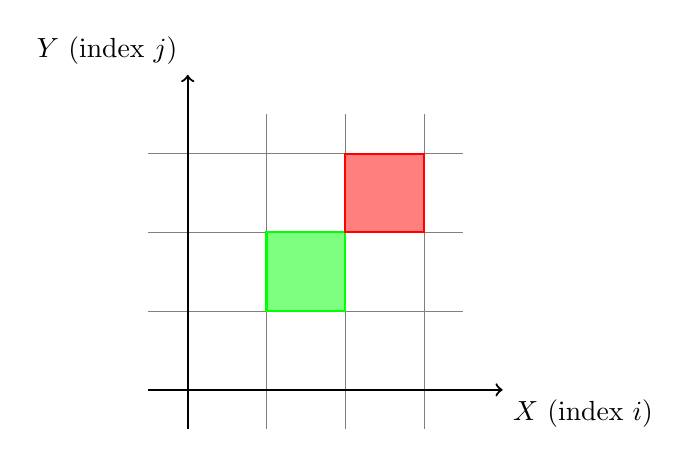
\begin{tikzpicture}
        % Draw the grid
        \draw[step=1cm,gray,very thin] (-0.5,-0.5) grid (3.5,3.5);    
        % Draw the axes
        \draw[thick,->] (-0.5,0) -- (4,0) node[anchor=north west] {$X$ (index $i$)};
        \draw[thick,->] (0,-0.5) -- (0,4) node[anchor=south east] {$Y$ (index $j$)};    
        % Draw the green square
        \filldraw[green, opacity=0.5] (1,1) rectangle (2,2);
        \draw[green, thick] (1,1) -- (2,1) -- (2,2) -- (1,2) -- cycle;    
        % Draw the red square
        \filldraw[red, opacity=0.5] (2,2) rectangle (3,3);
        \draw[red, thick] (2,2) -- (3,2) -- (3,3) -- (2,3) -- cycle;
        % % Add math notations
        % \node at (1,1) [below left] {$V_{i,j}$};
        % \node at (2,1) [below right] {$V_{i+1,j}$};
        % \node at (1,2) [above left] {$V_{i,j+1}$};
        % \node at (2,2) [above right] {$V_{i+1,j+1}$};
        
        % \node at (2,2) [below left] {$V_{i,j}$};
        % \node at (3,2) [below right] {$V_{i+1,j}$};
        % \node at (2,3) [above left] {$V_{i,j+1}$};
        % \node at (3,3) [above right] {$V_{i+1,j+1}$};        
    \end{tikzpicture}
    \end{center}    
    \begin{equation}
        \partial^2_{xy}V \approx \frac{1}{2\Delta x\Delta y} \left( \left(V_{i+1,j+1} - V_{i,j+1}\right)  - \left(V_{i+1,j}-V_{i,j}\right) + \left(V_{i,j}-V_{i-1,j}\right)  -  \left(V_{i, j-1}-V_{i-1,j-1}\right) \right)        
    \end{equation}
    Let $q =-\frac{1}{2\Delta x\Delta y}\rho\Omega$, we have
    \begin{equation}
        \rho\Omega\partial^2_{xy}V \approx q\left(\left(-V_{i+1, j+1}+ V_{i,j+1} \right) + \left(V_{i+1,j} - 2V_{i,j} + V_{i-1,j}\right) + \left(V_{i,j-1} - V_{i-1,j-1}\right) \right).     
    \end{equation}
    
    
    \item If $\rho < 0$, the up and down in spot and vol and the down and up in spot and vol are included. The corresponding cross matrix $\hat L$ will be different from the positive $\rho$ case.

    \begin{center}
    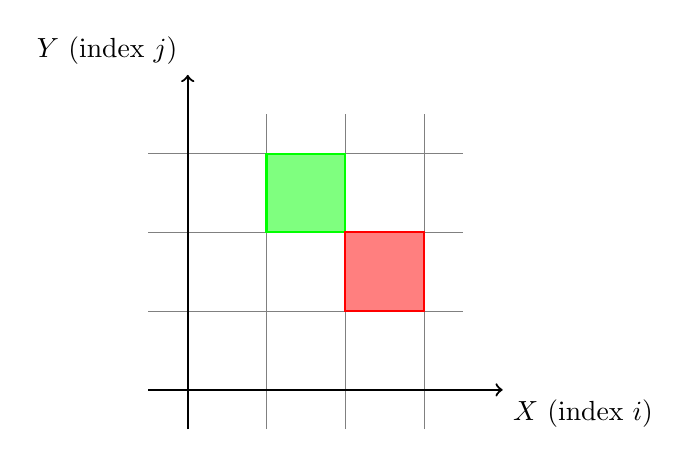
\begin{tikzpicture}    
        % Draw the grid
        \draw[step=1cm,gray,very thin] (-0.5,-0.5) grid (3.5,3.5);
        
        % Draw the axes
        \draw[thick,->] (-0.5,0) -- (4,0) node[anchor=north west] {$X$ (index $i$)};
        \draw[thick,->] (0,-0.5) -- (0,4) node[anchor=south east] {$Y$ (index $j$)};
        
        % Draw the green square
        \filldraw[green, opacity=0.5] (1,2) rectangle (2,3);
        \draw[green, thick] (1,2) -- (2,2) -- (2,3) -- (1,3) -- cycle;
        
        % Draw the red square
        \filldraw[red, opacity=0.5] (2,1) rectangle (3,2);
        \draw[red, thick] (2,1) -- (3,1) -- (3,2) -- (2,2) -- cycle;
        
        % Add math notations
        % \node at (2,2) [below left] {$V_{i,j}$};
        % \node at (3,2) [below right] {$V_{i+1,j}$};
        % \node at (2,3) [above left] {$V_{i,j+1}$};
        % \node at (3,3) [above right] {$V_{i+1,j+1}$};
        
        % \node at (3,1) [below left] {$V_{i,j-1}$};
        % \node at (4,1) [below right] {$V_{i+1,j-1}$};
        % \node at (3,2) [above left] {$V_{i,j}$};
        % \node at (4,2) [above right] {$V_{i+1,j}$};    
    \end{tikzpicture}
    \end{center}        
    % \begin{equation}
    %     \partial^2_{xy}V \approx \frac{1}{2\Delta x\Delta y} \left( \left(V_{i+1,j} - V_{i,j}\right)  - \left(V_{i+1,j-1}-V_{i,j-1}\right) + \left(V_{i,j+1}-V_{i-1,j+1}\right)  -  \left(V_{i, j}-V_{i,j-1}\right) \right)  
    % \end{equation}
    Similarly, let $q=-\frac{1}{2 \Delta x \Delta y} \rho \Omega$, we have
    \begin{equation}
        \rho\Omega\partial^2_{xy}V \approx q\left[\left(V_{i, j+1} - V_{i-1,j+1} \right) + \left(V_{i+1,j} - 2V_{i,j} + V_{i-1,j}\right) + \left(-V_{i+1,j-1} + V_{i,j-1}\right) \right]:
    \end{equation}    
    

    With the negative $\rho$, the cross matrix $\hat L$ is modified to
    \begin{equation}\label{eq: modified L_hat}
        \hat{L}=\left[\begin{array}{ccccc}L^{\prime} & Y & & & \\ Z & L^" & Y & & \\ & \cdots & \ldots & . . & \\ & & Z & L^" & Y \\ & & & Z & L^{"\prime }\end{array}\right],
    \end{equation}
    where the middle blocks are 
    
    \[
    L^" = \left[\begin{array}{cccccc}
    0 & 0 & & & & \\
    q & -2q & q & & & \\
    & q & -2q & q & & \\
    & & \cdots & \cdots & \cdots & \\
    & & & q & -2q & q \\
    & & & & 0 & 0
    \end{array}\right]
    \]
    
    \[
    Y = \left[\begin{array}{cccccc}
    0 & & & & & \\
    -q & q & & & & \\
    & -q & q & & & \\
    & & \cdots & \cdots & \cdots & \\
    & & & -q & q & \\
    & & & & & 0
    \end{array}\right]
    \]
    
    \[
    Z = \left[\begin{array}{cccccc}
    0 & & & & & \\
    & q & -q & & & \\
    & & q & -q & & \\
    & & \cdots & \cdots & \cdots & \\
    & & & & q & -q \\
    & & & & & 0
    \end{array}\right]
    \]

    the upper border is

    \[
    L^\prime = \left[\begin{array}{cccccc}
    0 & 0 & & & & \\
    q & -q & 0 & & & \\
    & q & -q & 0 & & \\
    & & \cdots & \cdots & \cdots & \\
    & & & q & -q & 0 \\
    & & & & 0 & 0
    \end{array}\right]
    \]

    the lower border is
     \[
    L^{"\prime} = \left[\begin{array}{cccccc}
    0 & 0 & & & & \\
    0 & -q & q & & & \\
    & 0 & -q & q & & \\
    & & \cdots & \cdots & \cdots & \\
    & & & 0 & -q & q \\
    & & & & 0 & 0
    \end{array}\right]
    \]
    
    In other words, compared to Eq (23) in JJ's work, in the negative $\rho$ case, we flipped these matrices along the diagonal.
    
\end{itemize}
\vspace{0.5cm}

    Below are eight graphs representing the transition matrix under flat local volatility. The four graphs in the left column correspond to the $\hat L$ matrix defined in JJ's work, with vol of vol ($\Omega$) set to $1 \times 10^{-4}$ and 0.75 , and $\rho$ values of $\pm 0.75$. The right column consists of four graphs that apply the modified $\hat{L}$ matrix defined in \eqref{eq: modified L_hat} , using the same choices of vol of vol and $\rho$.


    \begin{figure}[ht]
    \centering
    \begin{minipage}{0.45\textwidth}
        \centering
        \includegraphics[width=\textwidth]{fig/BEFORE Density plot with rho = 0.75, omega = 0.0001.jpg}
        \caption{[B] \(\Omega = 1 \times 10^{-4}\), \(\rho = 0.75\)}
    \end{minipage}
    \hfill
    \begin{minipage}{0.4\textwidth}
        \centering
        \includegraphics[width=\textwidth]{fig/AFTER Density plot with rho = 0.75, omega = 0.0001.jpg}
        \caption{[A] \(\Omega = 1 \times 10^{-4}\), \(\rho = 0.75\)}
    \end{minipage}

    \vspace{1em}

    \begin{minipage}{0.4\textwidth}
        \centering
        \includegraphics[width=\textwidth]{fig/BEFORE Density plot with rho = -0.75, omega = 0.0001.jpg}
        \caption{[B] \(\Omega  = 1 \times 10^{-4}\), \(\rho = -0.75\)}
    \end{minipage}
    \hfill
    \begin{minipage}{0.4\textwidth}
        \centering
        \includegraphics[width=\textwidth]{fig/AFTER Density plot with rho = -0.75, omega = 0.0001.jpg}
        \caption{[A] \(\Omega = 1 \times 10^{-4}\), \(\rho = -0.75\)}
    \end{minipage}

    \vspace{1em}

    \begin{minipage}{0.4\textwidth}
        \centering
        \includegraphics[width=\textwidth]{fig/BEFORE Density plot with rho = 0.75, omega = 0.75.jpg}
        \caption{[B] \(\Omega = 0.75\), \(\rho = 0.75\)} \label{fig: before change, 0.75 omega and 0.75 rho}
    \end{minipage}
    \hfill
    \begin{minipage}{0.4\textwidth}
        \centering
        \includegraphics[width=\textwidth]{fig/AFTER Density plot with rho = 0.75, omega = 0.75.jpg} 
        \caption{[A] \(\Omega = 0.75\), \(\rho = 0.75\)} \label{fig: after change, 0.75 omega and 0.75 rho}
    \end{minipage}

    \vspace{1em}

    \begin{minipage}{0.4\textwidth}
        \centering
        \includegraphics[width=\textwidth]{fig/BEFORE Density plot with rho = -0.75, omega = 0.75.jpg}
        \caption{[B] \(\Omega = 0.75\), \(\rho = -0.75\)} \label{fig: before change, 0.75 omega and -0.75 rho}
    \end{minipage}
    \hfill
    \begin{minipage}{0.4\textwidth}
        \centering
        \includegraphics[width=\textwidth]{fig/AFTER Density plot with rho = -0.75, omega = 0.75.jpg}
        \caption{[A] \(\Omega = 0.75\), \(\rho = -0.75\)} \label{fig: after change, 0.75 omega and -0.75 rho}
    \end{minipage}
\end{figure}
With the correctly identified cross matrix $\hat L$ , the transition density appears symmetric for both negative (Fig. \ref{fig: after change, 0.75 omega and -0.75 rho}) and positive (Fig. \ref{fig: before change, 0.75 omega and 0.75 rho}) $\rho$ cases under the flat LV tests. However, when an incorrectly identified cross matrix is applied, the transition density seems to exhibit skewness in both cases (positive $\rho$: Fig. \ref{fig: after change, 0.75 omega and 0.75 rho} and negative $\rho$: Fig. \ref{fig: before change, 0.75 omega and -0.75 rho}).




\end{document}


\end{document}
    